\section{Appendix}

\begin{table}[h]
\centering
\caption{Showcase of the \textbf{predictive performance} of both the informative and non-informative \texttt{Simple Temp.\ Model}}
\begin{tabularx}{\textwidth}{l l *{6}{>{\centering\arraybackslash}X} c c X}
\toprule
& \textbf{Model} & \multicolumn{2}{c}{\textbf{MAE}} & \multicolumn{2}{c}{\textbf{MSE}} & \multicolumn{2}{c}{\textbf{RMSE}} & \textbf{LPD} & \textbf{MAD} \\
\cmidrule(lr){3-4} \cmidrule(lr){5-6} \cmidrule(lr){7-8} 
& & Mean & Std & Mean & Std & Mean & Std & & \\
\midrule
\multirow{2}{*}{\rotatebox[origin=c]{90}{\tiny $\text{M}_1$-90}} 
& Valid & 0.485 & 0.077 & 0.371 & 0.111 & 0.601 & 0.090 & -21.399 & 0.317 \\
& Test & 0.530 & 0.097 & 0.428 & 0.146 & 0.645 & 0.109 & -23.615 & 0.396 \\ [0.2ex]
\cmidrule(lr){2-10}
\multirow{2}{}{\rotatebox[origin=c]{90}{\tiny $\text{M}_1$-180}}
& Valid & 0.551 & 0.083 & 0.487 & 0.135 & 0.691 & 0.097 & -25.821 & 0.385 \\
& Test & 0.750 & 0.098 & 0.801 & 0.187 & 0.889 & 0.104 & -39.710 & 0.691 \\ [0.2ex]
\cmidrule(lr){2-10}
\multirow{2}{}{\rotatebox[origin=c]{90}{\tiny $\text{M}_1$-365}}
& Valid & 0.677 & 0.106 & 0.720 & 0.212 & 0.839 & 0.125 & -27.358 & 0.378 \\
& Test & 0.627 & 0.103 & 0.616 & 0.189 & 0.776 & 0.120 & -25.094 & 0.314 \\ [0.2ex]
\cmidrule(lr){2-10}
\multirow{2}{}{\rotatebox[origin=c]{90}{\tiny $\text{M}_1$-1166}}
& Valid & 1.135 & 0.167 & 1.932 & 0.514 & 1.378 & 0.185 & -41.221 & 0.920 \\
& Test & 1.240 & 0.172 & 2.194 & 0.542 & 1.470 & 0.183 & -44.422 & 1.118 \\ [0.4ex]
\cmidrule(lr){2-10}
\multirow{2}{*}{\rotatebox[origin=c]{90}{\tiny $\text{M}_1^i$-90}}
& Valid & 0.482 & 0.078 & 0.370 & 0.111 & 0.601 & 0.091 & -21.259 & 0.316 \\
& Test & 0.528 & 0.093 & 0.426 & 0.139 & 0.644 & 0.106 & -23.534 & 0.394 \\ [0.2ex]
\cmidrule(lr){2-10}
\multirow{2}{}{\rotatebox[origin=c]{90}{\tiny $\text{M}_1^i$-180}}
& Valid & 0.550 & 0.081 & 0.482 & 0.133 & 0.688 & 0.095 & -25.489 & 0.385 \\
& Test & 0.730 & 0.097 & 0.760 & 0.181 & 0.865 & 0.104 & -37.828 & 0.667 \\ [0.2ex]
\cmidrule(lr){2-10}
\multirow{2}{}{\rotatebox[origin=c]{90}{\tiny $\text{M}_1^i$-365}}
& Valid & 0.673 & 0.107 & 0.712 & 0.210 & 0.835 & 0.124 & -27.209 & 0.372 \\
& Test & 0.628 & 0.104 & 0.617 & 0.192 & 0.776 & 0.121 & -25.097 & 0.310 \\ [0.2ex]
\cmidrule(lr){2-10}
\multirow{2}{*}{\rotatebox[origin=c]{90}{\tiny $\text{M}_1^i$-1166}}
& Valid & 1.135 & 0.162 & 1.930 & 0.503 & 1.378 & 0.180 & -41.226 & 0.920 \\
& Test & 1.235 & 0.173 & 2.180 & 0.540 & 1.465 & 0.183 & -44.571 & 1.117 \\ [0.5ex]
\bottomrule
\end{tabularx}
\label{tab:temp_models_full_performance}
\end{table}

\begin{table}[h]
\centering
\caption{Comparison of predicted and true daily means for the test, as forecasted by the \texttt{Hybrid Model} $M4{-}90{-}1166$. The last column shows the difference between the predicted and true values, providing a measure of the model's accuracy.}
\label{tab:hybrid_preds}
\begin{tabular}{cccc}
\toprule
Date       & Predicted Mean & True Mean & Difference \\ \midrule
2023-04-03 & -0.0694       & 0.0044    & -0.0737    \\
2023-04-04 & 0.2631        & 0.2380    & 0.0251     \\
2023-04-05 & 0.5011        & 1.0929    & -0.5918    \\
2023-04-06 & 1.0561        & 0.8853    & 0.1708     \\
2023-04-07 & 1.0651        & 1.1716    & -0.1065    \\
2023-04-08 & 0.6112        & 0.6580    & -0.0468    \\
2023-04-09 & 0.3057        & 0.4934    & -0.1877    \\
2023-04-10 & 0.2772        & -0.3859   & 0.6631     \\
2023-04-11 & 0.1697        & 0.4818    & -0.3121    \\
2023-04-12 & 0.5725        & 0.4580    & 0.1145     \\
2023-04-13 & 0.8907        & 0.9496    & -0.0589    \\
2023-04-14 & 1.1156        & 1.3092    & -0.1936    \\
2023-04-15 & 0.8320        & 0.2265    & 0.6055     \\
2023-04-16 & -0.0343       & 0.4226    & -0.4569    \\
2023-04-17 & 0.2496        & -0.1679   & 0.4175     \\
2023-04-18 & 0.1360        & 0.4906    & -0.3546    \\
2023-04-19 & 0.6742        & 1.0130    & -0.3388    \\
2023-04-20 & 0.8489        & 1.1565    & -0.3076    \\
2023-04-21 & 1.1375        & 2.1284    & -0.9909    \\
2023-04-22 & 1.1266        & 1.2983    & -0.1717    \\
2023-04-23 & 1.0199        & 0.7563    & 0.2636     \\ \bottomrule
\end{tabular}
\end{table}


\begin{figure}[h!]
    \centering
    \begin{subfigure}[b]{0.3\textwidth}
        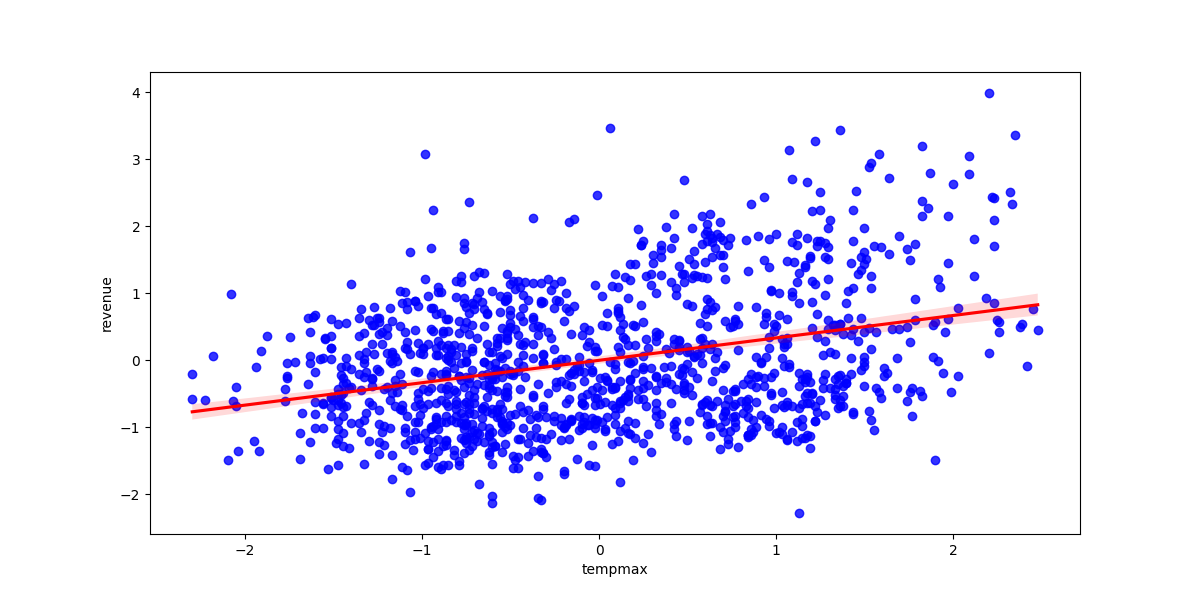
\includegraphics[width=\textwidth]{../../preprocessing/plots/tempmax.png}
        \caption{Correlation with temperature}
    \end{subfigure}
    \begin{subfigure}[b]{0.3\textwidth}
        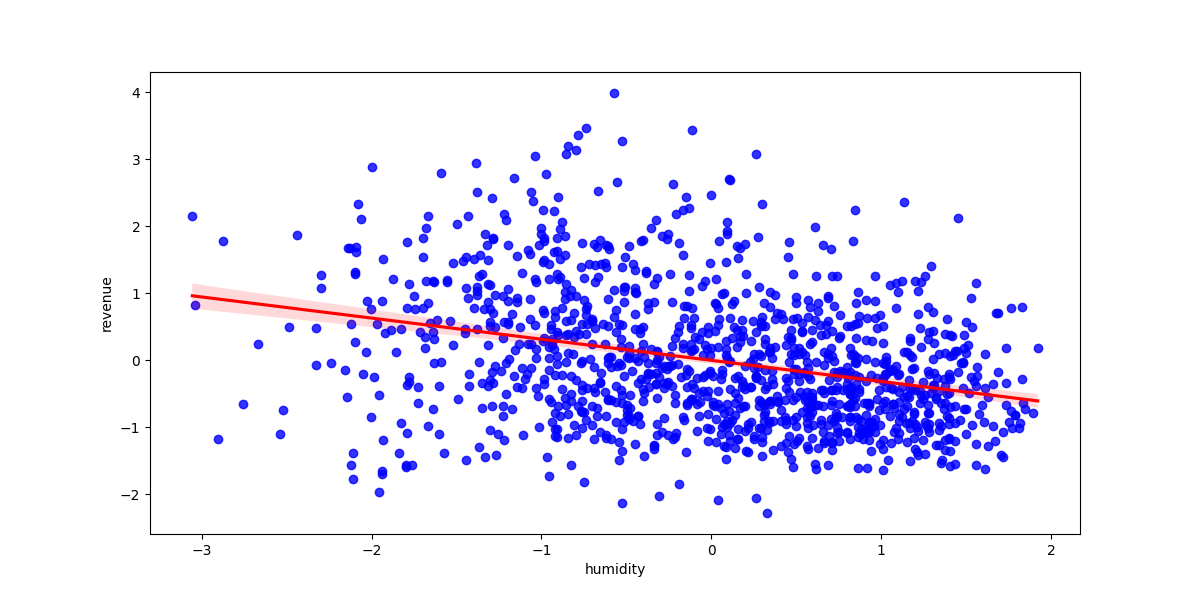
\includegraphics[width=\textwidth]{../../preprocessing/plots/humidity.png}
        \caption{Correlation with humidity}
    \end{subfigure}
    \begin{subfigure}[b]{0.3\textwidth}
        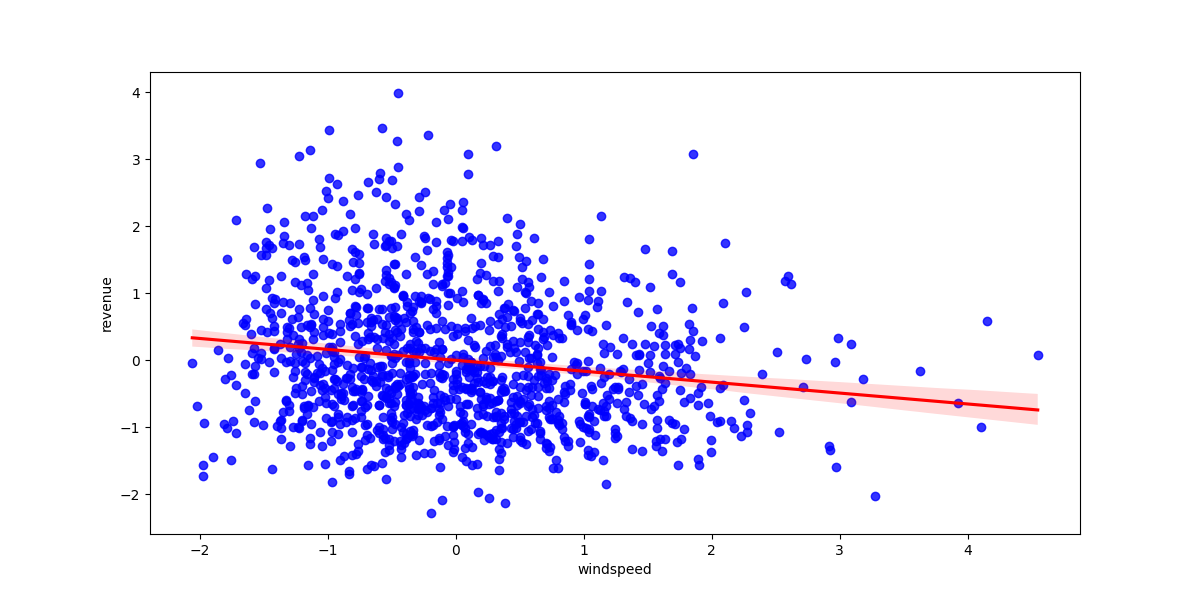
\includegraphics[width=\textwidth]{../../preprocessing/plots/windspeed.png}
        \caption{Correlation with windspeed}
    \end{subfigure}
    \begin{subfigure}[b]{0.3\textwidth}
        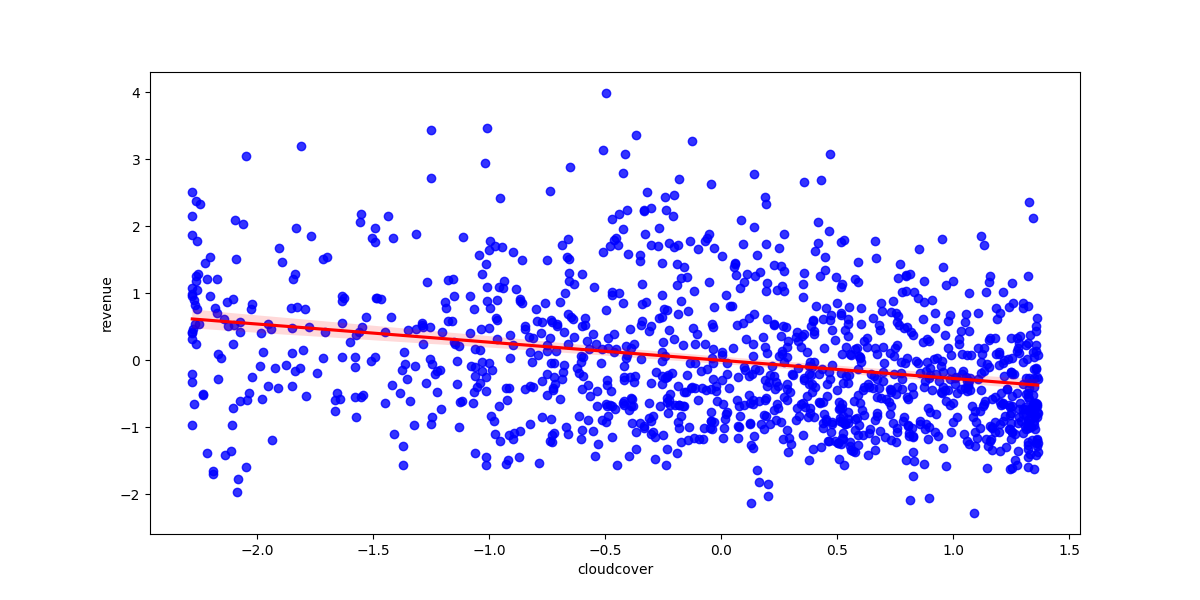
\includegraphics[width=\textwidth]{../../preprocessing/plots/cloudcover.png}
        \caption{Correlation with cloudcover}
    \end{subfigure}
    ~ % add extra space
    \begin{subfigure}[b]{0.3\textwidth}
        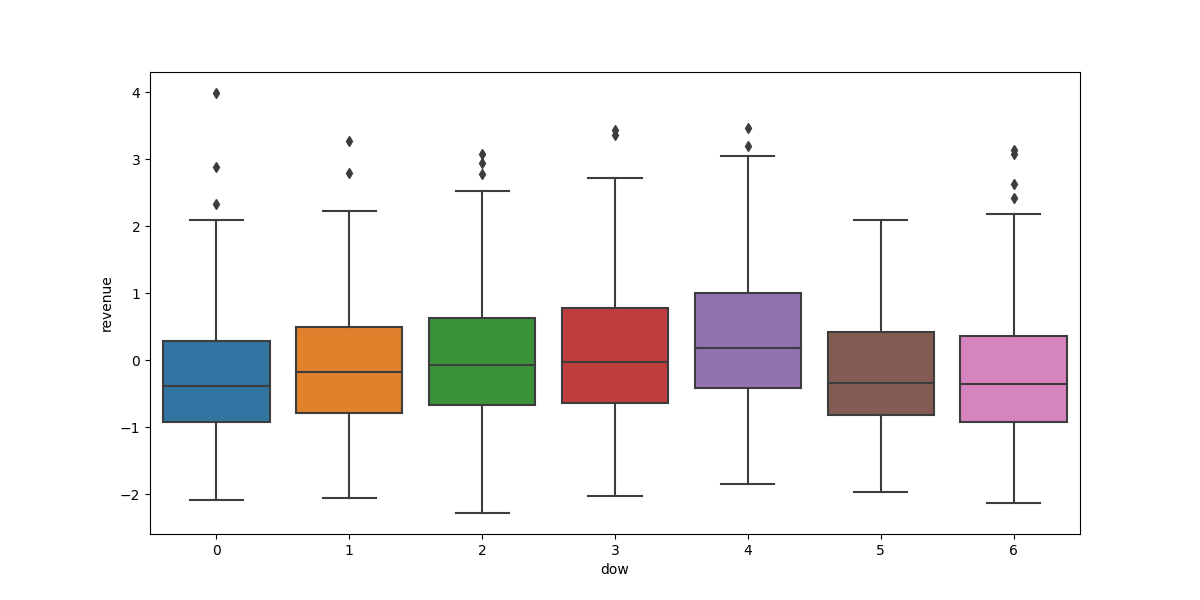
\includegraphics[width=\textwidth]{../../preprocessing/plots/dow.png}
        \caption{Correlation with day of week}
    \end{subfigure}
    \begin{subfigure}[b]{0.3\textwidth}
        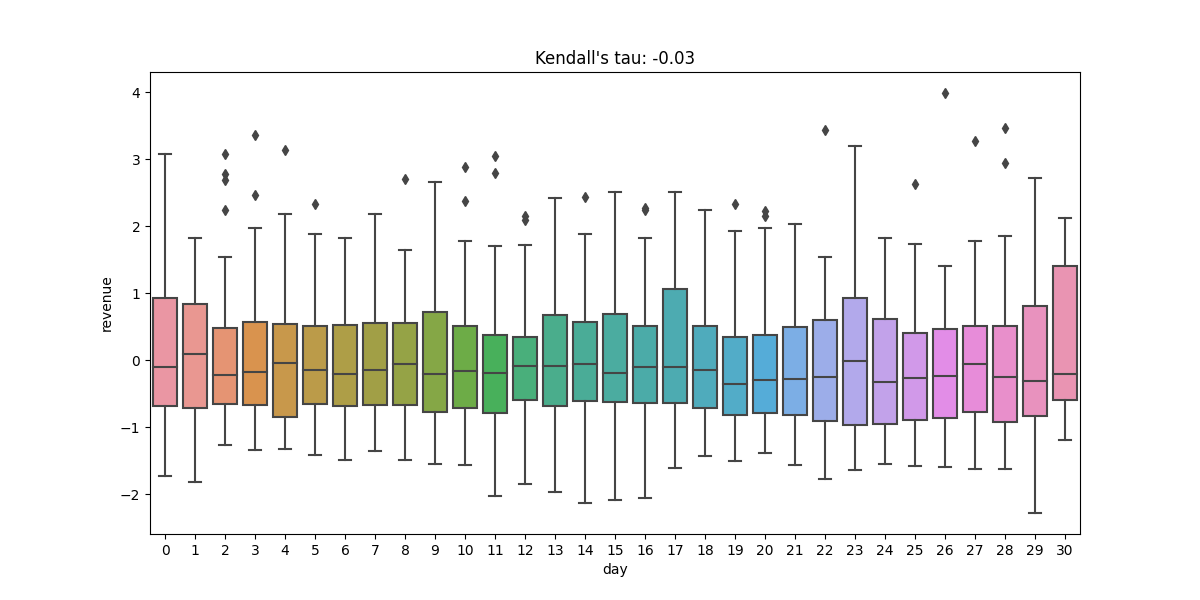
\includegraphics[width=\textwidth]{../../preprocessing/plots/day.png}
        \caption{Correlation with day}
    \end{subfigure}
    ~ % add extra space
    \begin{subfigure}[b]{0.3\textwidth}
        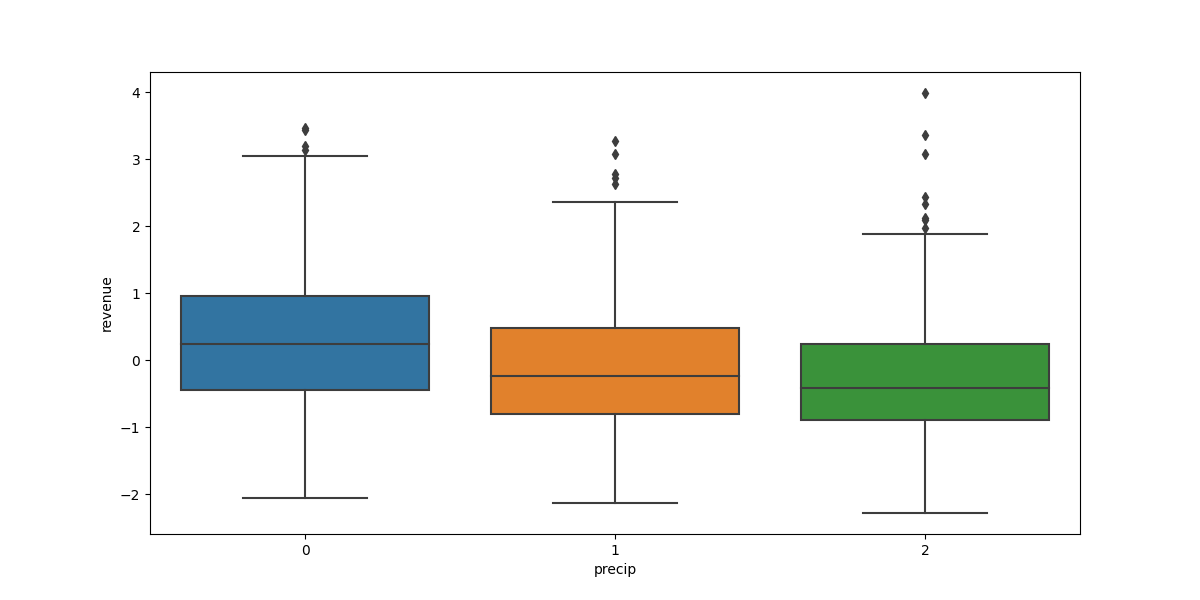
\includegraphics[width=\textwidth]{../../preprocessing/plots/precip.png}
        \caption{Correlation with precipitation}
    \end{subfigure}
    \begin{subfigure}[b]{0.3\textwidth}
        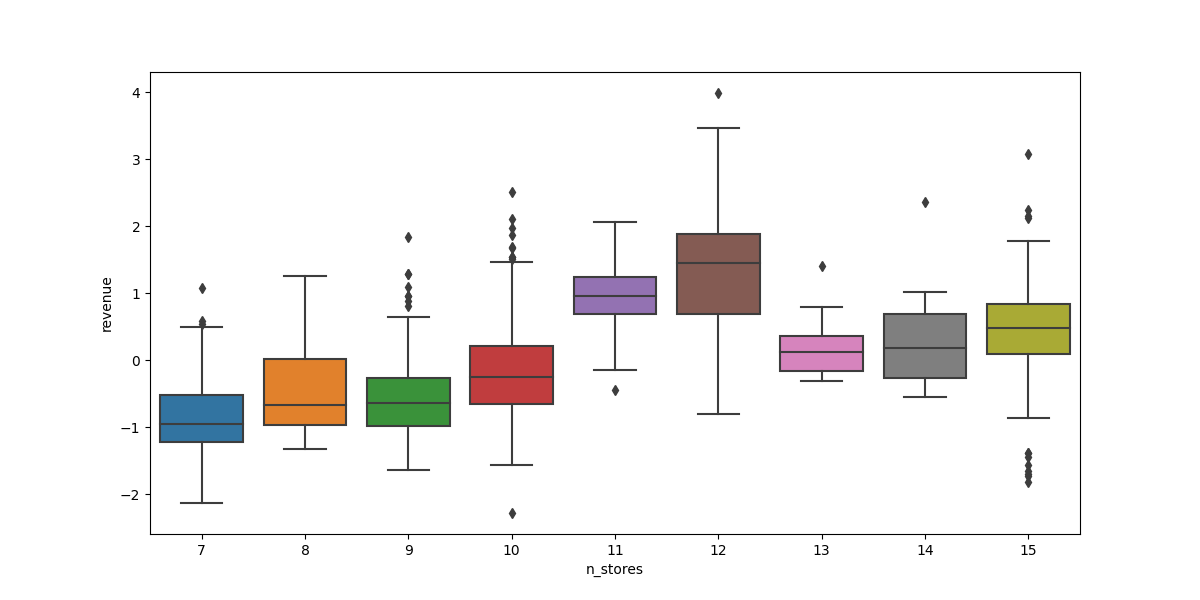
\includegraphics[width=\textwidth]{../../preprocessing/plots/n_stores.png}
        \caption{Correlation with number of stores}
    \end{subfigure}
    \begin{subfigure}[b]{0.3\textwidth}
        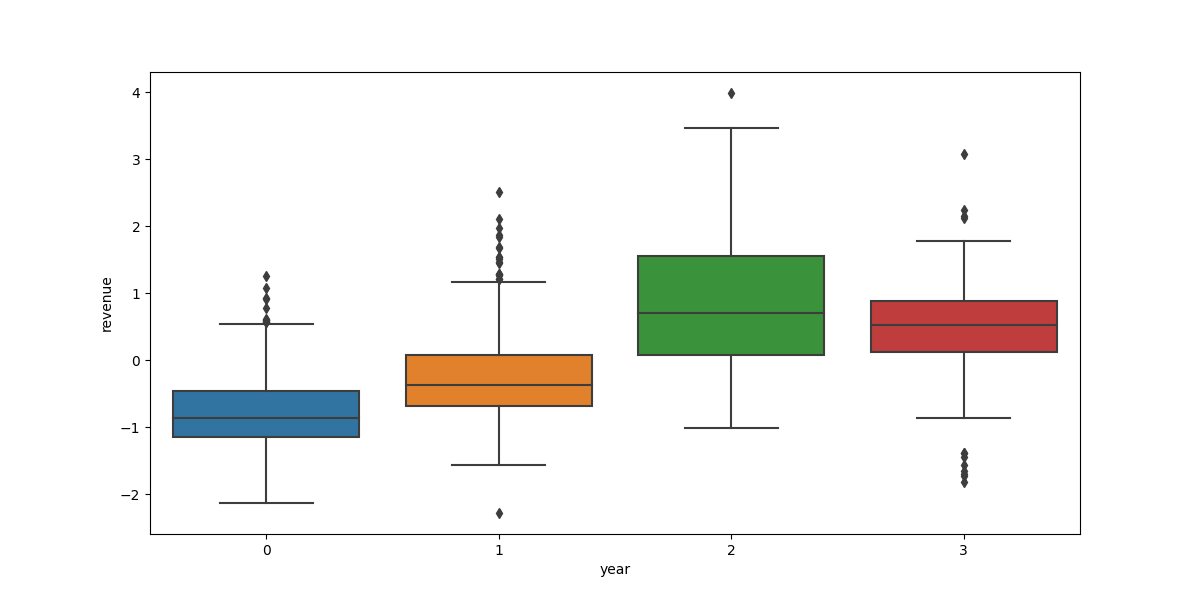
\includegraphics[width=\textwidth]{../../preprocessing/plots/year.png}
        \caption{Correlation with year}
        \label{fig:corr_year}
    \end{subfigure}
    \begin{subfigure}[b]{0.3\textwidth}
        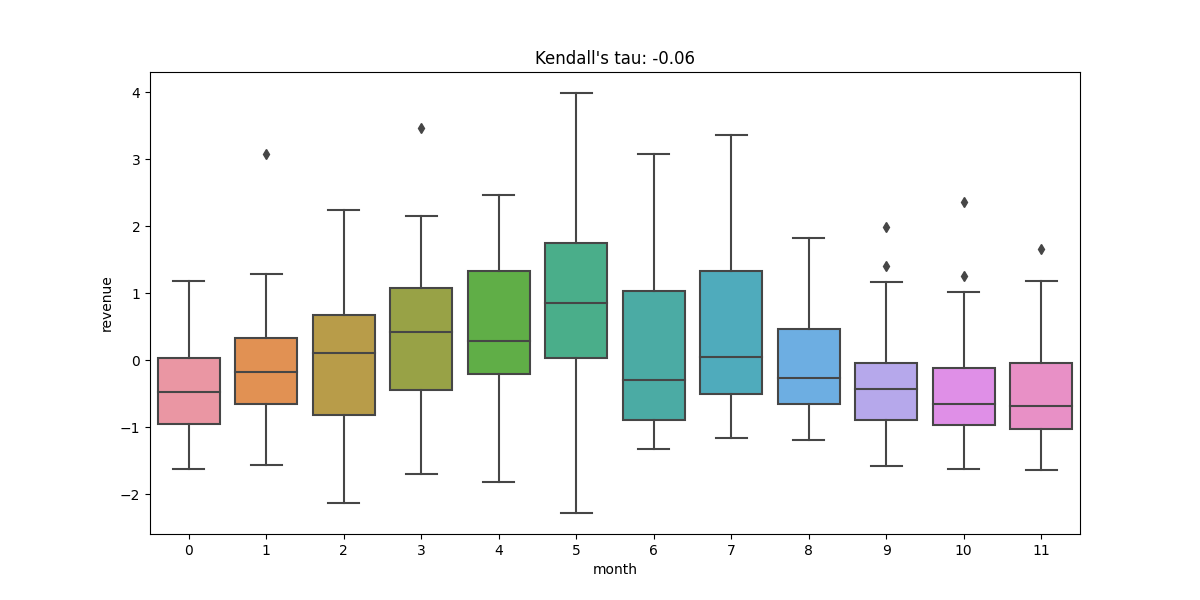
\includegraphics[width=\textwidth]{../../preprocessing/plots/month.png}
        \caption{Correlation with month}
        \label{fig:corr_year}
    \end{subfigure}
    \caption{Correlation analysis of different predictors. Each subplot represents the correlation of the daily revenue with a specific predictor.}
    \label{fig:corr_analysis}
\end{figure}

